\section{Introduction}
A graph is an \emph{intersection graph} if every vertex can be assigned with a set such that there is an edge between two vertices if their corresponding sets intersect. The class of \emph{interval graphs} (see Figure \ref{interval_graph}) is a special type of intersection graphs when sets are line segments on a line. The study of interval graphs arises naturally in solving real-world problems. The line on which the intervals rest may represent a period of time, a range of temperatures, or an interval of DNA. Many problems can be reduced to the recognition of interval graphs. Interval graphs are useful mathematical structures in genetics, bioinformatics, and various resource allocation problems.

\begin{figure}[H]
\centering
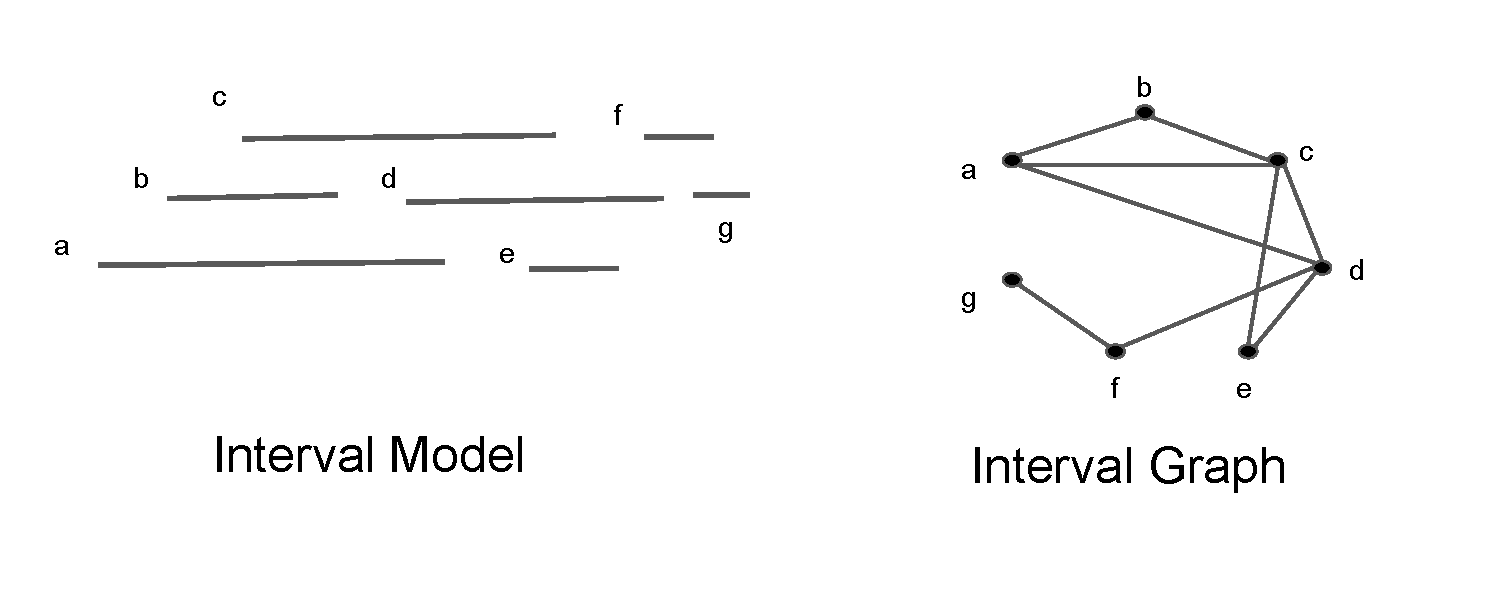
\includegraphics[width=12cm,height=6cm]{figures/interval_graph.pdf}
\caption{An example of an interval graph}
\label{interval_graph}
\end{figure}


Interval graphs have close connections to many other important graph classes such as chordal graphs, comparability graphs, and circular-arc graphs. A graph is \emph{chordal} if every cycle of length four or greater possesses a \empy{chord}, that is, an edge joining two nonconsecutive vertices of the cycle. Interval graphs are a subfamily of chordal graphs. If a graph is not chordal, it fails to be an interval graph. Furthermore, the linear time recognition algorithm of interval graphs relies on the fact that the number of cliques in a chordal graph is polynomial. Therefore, as the first step, the recognition algorithm of interval graph checks whether it is a chordal graph. Properties and recognition algorithm of chordal graphs will be in Section \ref{chordal} in more details. A \emph{comparability graph} is an undirected graph where adjacent pairs of elements are comparable to each other in a partial order. Gilmore and Hoffman\cite{gilmore1964characterization} show that an undirected graph $G$ is an interval graph if and only if $G$ is chordal and its complement, $\bar{G}$, is a comparability graph. 

A \emph{maximal clique} is a clique that cannot be extended to a larger clique by including one more vertex. A \emph{clique matrix} (see Figure \ref{cons_ones}) is a matrix such that the entry in row $i$ column $j$ is $1$ if vertex $i$ is a member of clique $j$. A \emph{consecutive-ones ordering}(in Figure \ref{cons_ones}) of the clique matrix is a permutation of the columns to make 1's occur consecutively in each row. A matrix has the \emph{consecutive-ones property} if there exists such an ordering of the columns.

Fulkerson and Gross\cite{fulkerson1965incidence} prove that an undirected graph is an interval graph if and only if its clique matrix M has the consecutive-ones property. Booth and Leuker\cite{booth1976testing} demonstrate a linear time recognition algorithm for interval graphs based on a data structure called a \emph{PQ tree}, which is a tree-based data structure that represents a family of permutations on a set of elements. Their method follows the idea of narrowing down the permitted permutations while adding each row, and a PQ tree representing all possible consecutive-ones orderings of the clique matrix is maintained. Several other algorithms\cite{corneil2009lbfs}\cite{habib2000lex}\cite{mcconnell2009linear} have been proposed after that for simpler implementations.

\begin{figure}[H]
\centering
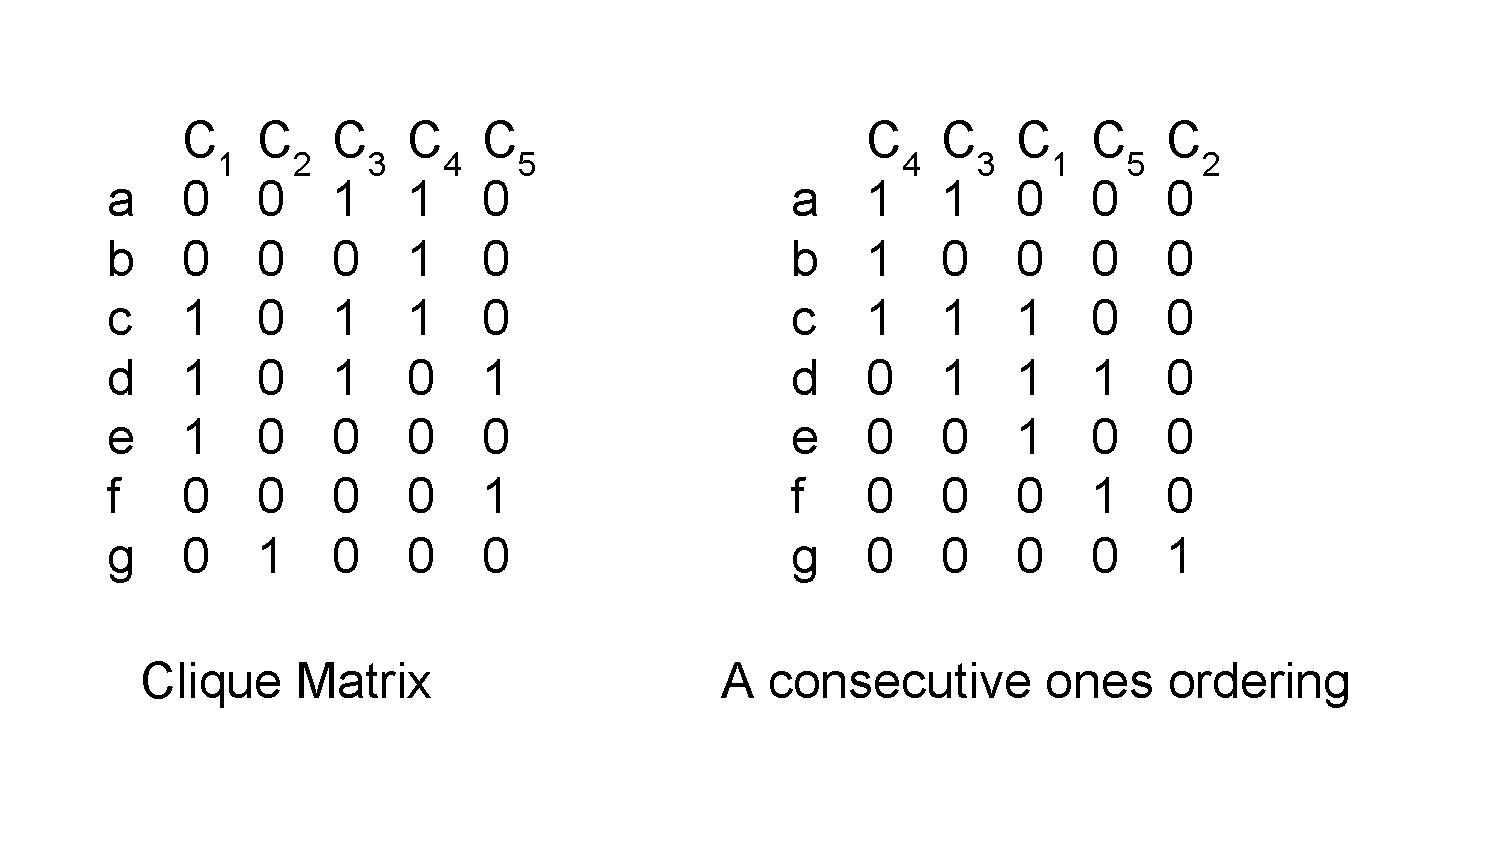
\includegraphics[width=12cm,height=6cm]{figures/cons_ones.pdf}
\caption{Clique Matrix and Consecutive-ones ordering. Maximal cliques $C_1: \{c,d,e\}$, $C_2: \{f,g\}$, $C_3: \{a,c,d\}$, $C_4: \{a,b,c\}$, $C_5: \{d,f\}.$}
\label{cons_ones}
\end{figure}

Certifying algorithms originate from the need to protect software compromised by undetected bugs. As algorithms get more complicated, the users get less likely to know whether the final solution is correct or the software is potentially compromised by a bug. Therefore, we need a certificate for the output of the algorithm. The certificate should be easy to check and with the size less than the input. The certificate is useful while designing reliable software. A \emph{certifying algorithm} is an algorithm that not only outputs a solution but also outputs an easy-to-verify proof to its solution. This easy-to-verify proof together with a checking algorithm is called a certificate. As an example, it is a well-known fact that a graph is a bipartite graph if and only if it does not contain an odd cycle. Therefore, a certifying algorithm for recognizing bipartite graphs can be one that outputs a partition of the vertices if the graph is a bipartite graph, or an odd cycle if it fails to be bipartite. The certificate easily allows us to verify whether the edges are between the two partitions, or to verify that the odd cycle exists in the given graph.

In recognition algorithms, forbidden structures are usually regarded as certificates due to their simplicity for verifying. Many important families of graphs can be characterized with \emph{forbidden structures} as follows: a graph $G$ is in the family if and only if it does not contain a forbidden structure. A classic example is about planar graphs, which are graphs that can be embedded in a plane such that its edges intersect only at vertices. A \emph{subdivision} of a graph is a graph formed by subdividing its edges into paths of one or more edges. A graph is planar if and only if it does not contain a \emph{Kuratowski subgraph}(see Figure \ref{kura_subgraph}), which is a subdivision of complete graph $K_5$ or bipartite complete graph $K_{3,3}$. 

\begin{figure}[H]
\centering
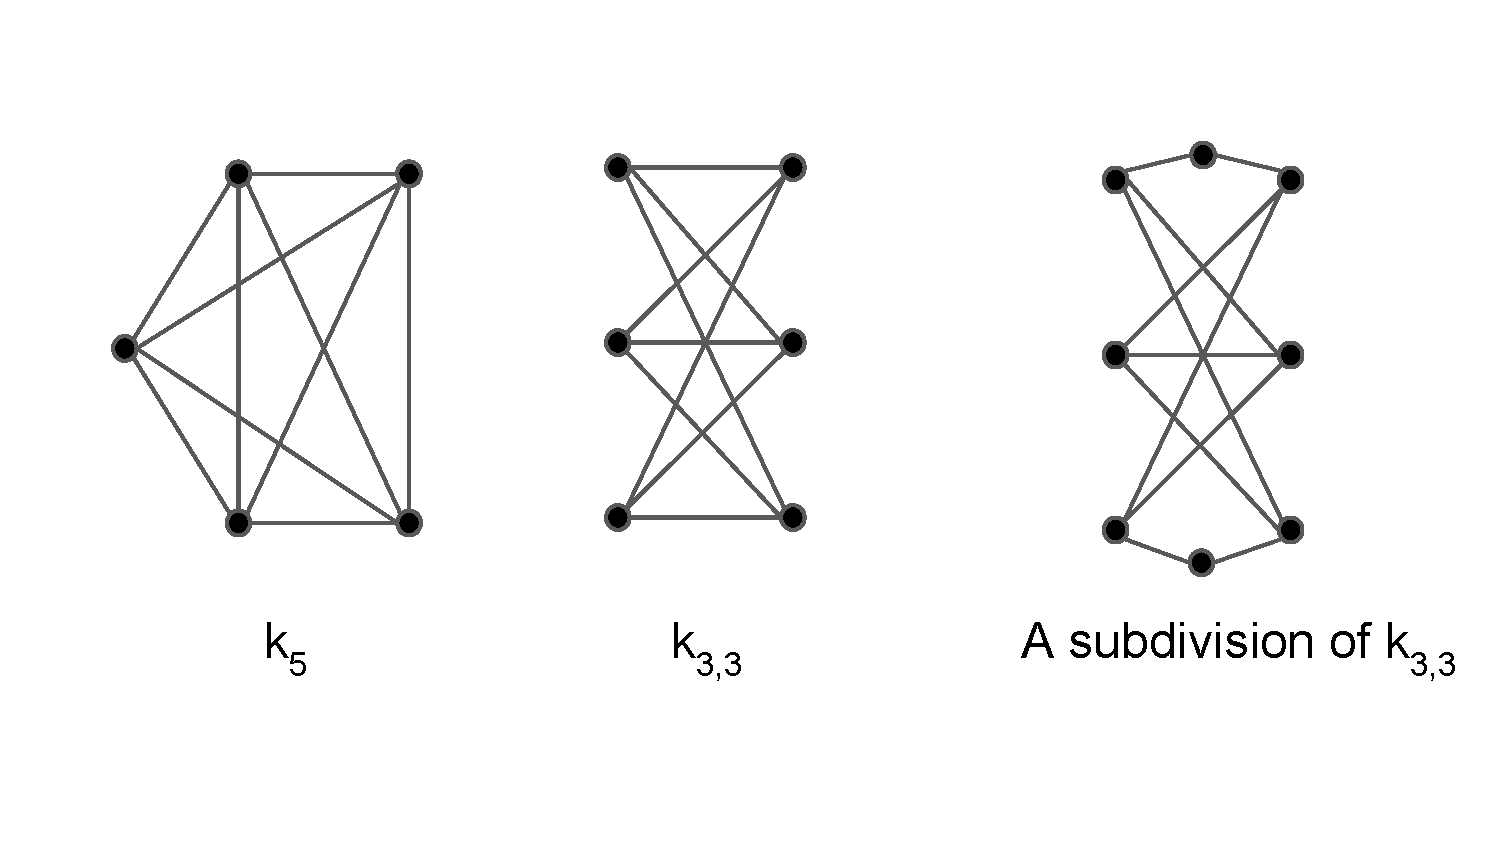
\includegraphics[width=12cm]{figures/kura_subgraph.pdf}
\caption{Example of Kuratowski subgraphs}
\label{kura_subgraph}
\end{figure}

The first forbidden structure characterization of interval graphs  pointed out by Lekerkerker and Boland(1962)\cite{lekkerkerker1962representation} that an undirected graph is an interval graph if and only if it is chordal and does not contain a \emph{Asteroidal Triple} ("$AT$"), which is three independent vertices such that there is a path between every two vertices that avoids any neighbor of the third vertex. Thereby, they derive the forbidden induced subgraphs for interval graphs (see Figure \ref{lb_subgraph}). Tucker\cite{tucker1972structure} also gives the forbidden submatrices for a matrix that has the consecutive-ones property (see Figure \ref{tucker_matrix}). Lindzey and McConnell(2016)\cite{lindzey2016linear} give a linear time algorithm for finding one of Tucker's submatrices in a matrix M that does not have the consecutive-ones property. A linear time algorithm for finding an induced LB subgraph is also included, thereby giving a linear time certifying recognition algorithm for interval graphs.

\begin{figure}[H]
\centering
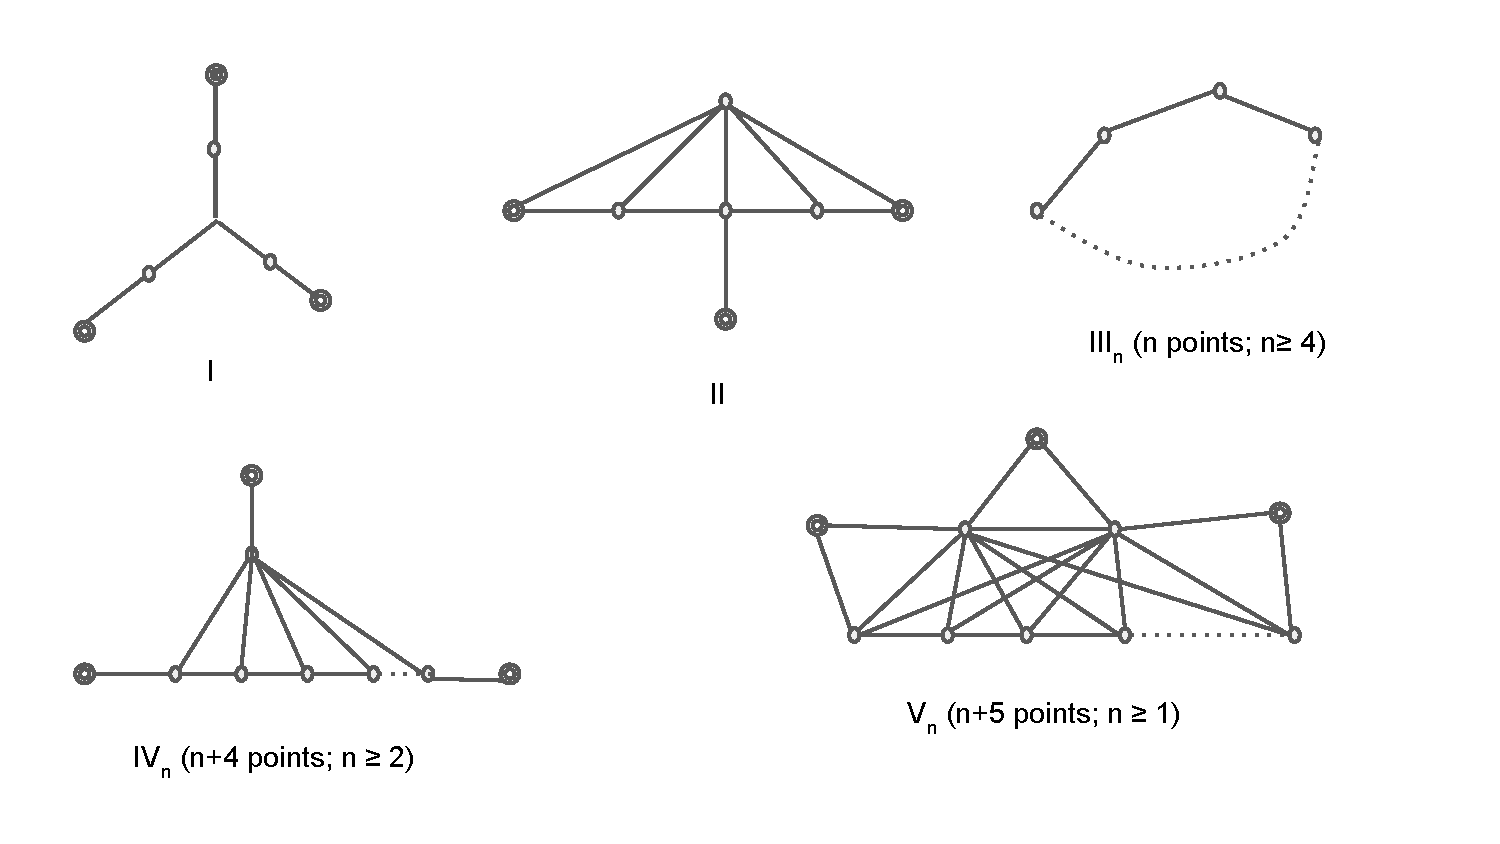
\includegraphics[width=12cm]{figures/lb_subgraph.pdf}
\caption{Lekerkerker-Boland(LB) Subgraphs}
\label{lb_subgraph}
\end{figure}

\begin{figure}[H]
\centering
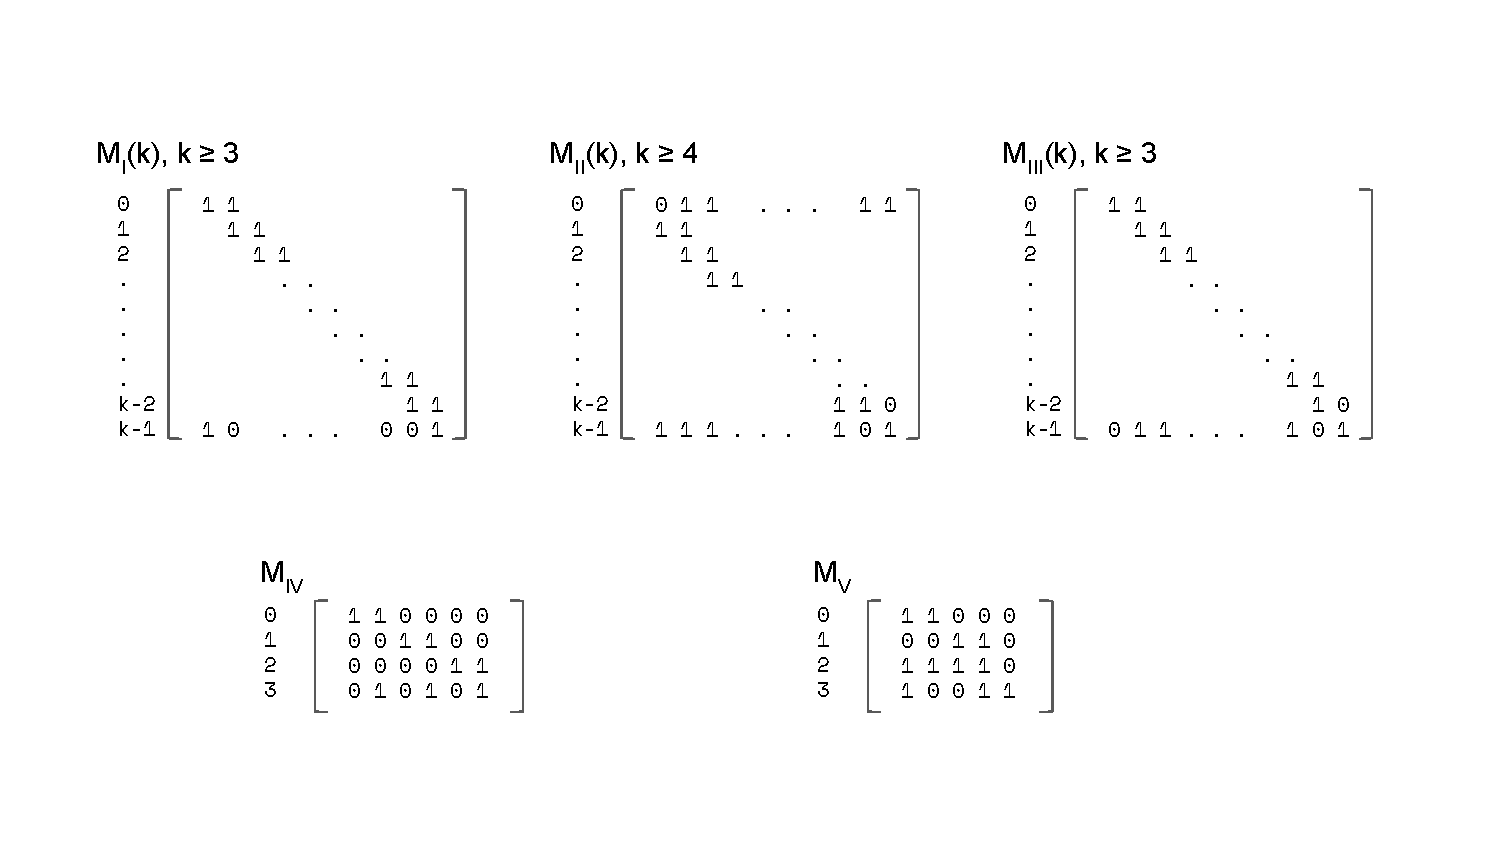
\includegraphics[width=16cm]{figures/tucker_matrix.pdf}
\caption{The minimal forbidden submatrices for consecutive-ones matrices(Tucker Matrices)}
\label{tucker_matrix}
\end{figure}











